\documentclass[xcolor=dvipsnames]{beamer}

\geometry{paperwidth=140mm,paperheight=105mm}

\usepackage[utf8x]{inputenc}
\usepackage{amsmath,amsfonts,amssymb}
\usecolortheme{default}
\usepackage{graphicx}
\usepackage{tikz}
\usepackage{caption}
\usepackage{nicefrac}
\usepackage{mathabx}
\usepackage{hyperref}
%\usepackage{wrapfig}
% %\usepackage{cutwin}

\definecolor{DarkBlue}{HTML}{002e77}

\newcommand{\averx}{\langle x \rangle}
\newcommand{\Raverx}{\averx_\mathrm{ren}}

\usetheme{Boadilla}
\usecolortheme[named=DarkBlue]{structure}
\useinnertheme{rounded}

\usefonttheme{professionalfonts}
\setbeamertemplate{navigation symbols}{}
\setbeamertemplate{enumerate items}[square]

\usepackage{algorithm}
\usepackage{algorithmicx}
\usepackage{algpseudocode}

\makeatletter
\renewcommand{\ALG@beginalgorithmic}{\small}
\makeatother

\usepackage{sourcecodepro}
\usepackage{listings}
\definecolor{mygreen}{rgb}{0,0.6,0}
\definecolor{mygray}{rgb}{0.5,0.5,0.5}
\definecolor{mymauve}{rgb}{0.58,0,0.82}
% \PassOptionsToPackage{svgnames}{xcolor}

\lstset{ %
  backgroundcolor=\color{white},   % choose the background color; you must add \usepackage{color} or \usepackage{xcolor}; should come as last argument
  basicstyle=\footnotesize\ttfamily, % the size of the fonts that are used for the code
  breakatwhitespace=false,         % sets if automatic breaks should only happen at whitespace
  breaklines=true,                 % sets automatic line breaking
  captionpos=b,                    % sets the caption-position to bottom
  commentstyle=\color{mygreen},    % comment style
  deletekeywords={...},            % if you want to delete keywords from the given language
  escapeinside={\%*}{*)},          % if you want to add LaTeX within your code
  extendedchars=false,              % lets you use non-ASCII characters; for 8-bits encodings only, does not work with UTF-8
  frame=single,	                   % adds a frame around the code
  keepspaces=true,                 % keeps spaces in text, useful for keeping indentation of code (possibly needs columns=flexible)
  keywordstyle=\color{blue},       % keyword style
  language=C,                      % the language of the code
  morekeywords={*,...},            % if you want to add more keywords to the set
  numbers=none,                    % where to put the line-numbers; possible values are (none, left, right)
  numbersep=5pt,                   % how far the line-numbers are from the code
  numberstyle=\tiny\color{mygray}, % the style that is used for the line-numbers
  rulecolor=\color{black},         % if not set, the frame-color may be changed on line-breaks within not-black text (e.g. comments (green here))
  showspaces=false,                % show spaces everywhere adding particular underscores; it overrides 'showstringspaces'
  showstringspaces=false,          % underline spaces within strings only
  showtabs=false,                  % show tabs within strings adding particular underscores
  stepnumber=1,                    % the step between two line-numbers. If it's 1, each line will be numbered
  stringstyle=\color{mymauve},     % string literal style
  tabsize=2,	                   % sets default tabsize to 2 spaces
  moredelim=**[is][\color{red}]{!@}{!@},
  %title=\lstname                   % show the filename of files included with \lstinputlisting; also try caption instead of title
}

\renewcommand{\UrlFont}{\small}

\newcounter{lecturecounter}
\setcounter{lecturecounter}{1}

\author[B. Kostrzewa]{Bartosz Kostrzewa, Ferenc Pittler, Martin Ueding, Carsten Urbach}
\title{C-Kurs Physik, 2017}
\institute[HISKP]{HISKP, Rheinische Friedrich-Wilhelms-Universität Bonn}
% \titlegraphic{\roundbox{\includegraphics[height=2cm]{UniBonn_CRC110_ETMC_INFN}}}
\date[April 2017]{April 2017}

\begin{document}

% \frame{}
\begin{frame}
 \titlepage
\end{frame}

\begin{frame}{Administrativa}
  \begin{itemize}
  \item{Vorlesung 03.04-13.04, 10-12 Uhr, \textbf{PI HS1}}
  \begin{itemize}
    \item{06.04: \textbf{HS HISKP} }
  \end{itemize}
  \vspace{0.2cm}
  \item{Bartosz Kostrzewa, bartosz\_kostrzewa@fastmail.com, Raum 3.009 HISKP}
  \begin{itemize}
    \item{Sprechzeiten: Täglich 17:00-17:45 Uhr}
  \end{itemize}
  \vspace{0.2cm}
  \item{Tutoren}
  \begin{itemize}
    \item{Martin~Ueding, Simon~Schlepphorst, 
         \\Ferenc~Pittler, Marcel~Nitsch, Florian~Tauber} 
  \end{itemize}
  \vspace{0.2cm}
  \item{Tutorien finden statt: täglich 13:00-17:00}
  \begin{itemize}
    \item{Astro CIP Pool (Raum 0.007) [AifA, Auf dem Hügel 71]}
    \item{HISKP SR1 [HISKP, Nußallee 14-16]}
    \begin{itemize}
      \item{\textbf{ $\mathbf{18}$ Personen $\rightarrow$ Astro, $\quad\mathbf{N-18}$ $\rightarrow$ SR1} }
    \end{itemize}
  \end{itemize}
  \vspace{0.2cm}
  \item{Das Skript dient als Referenz und sollte zumindest während der Tutorien befragt werden!}
  \vspace{0.2cm}
  \item{Fundamentale Ungleichung der Programmierung (FUP!): \\ \textbf{Praxis $\mathbf{\gg}$ Vorlesungen} $\rightarrow$ besuchen Sie die Übungen, sonst bringt die Vorlesung nichts!}
  \item{Folien und Übungszettel: \textcolor{blue}{\url{http://goo.gl/xhJN08}}}
  \end{itemize}
\end{frame}

\begin{frame}{Lernziele}
\begin{itemize}
  \item{Algorithmen verstehen und entwickeln}
  \item{Algorithmen in Quelltext übertragen}
  \vspace{0.3cm}
  \item{Erstes Kennenlernen der sogennanten \emph{imperativen} Programmierung}
  \item{Kennenlernen der Daten- und Kontrollstrukturen von C99}
  \vspace{0.3cm}
  \item{Praktischer Einsatz des C-Compilers zur Übersetzung des Quelltextes in ausführbaren Maschinencode}
  \item{Erstellen eigener C-Programme in den Tutorien}
  \begin{itemize}
    \item{einfache Beispielprogrammen $\rightarrow$ kompliziertere Programme aus merheren Quelltextdateien}
    \item{Verwendung externer Bilbiotheken}
  \end{itemize}
  \vspace{0.3cm}
  \item{Vorbereitung auf \emph{physik441: Computerphysik} (SoSe 2017), \emph{physics760: Computational Physics} (WiSe 2017/2018), etwaige Bachelor- und Masterarbeiten}
\end{itemize} 
\end{frame}

\begin{frame}{Anwendung: Plasmaphysik / Fusion}
  \centering
  Wellenstein 7-x Stellerator\\ \vspace{0.2cm}
  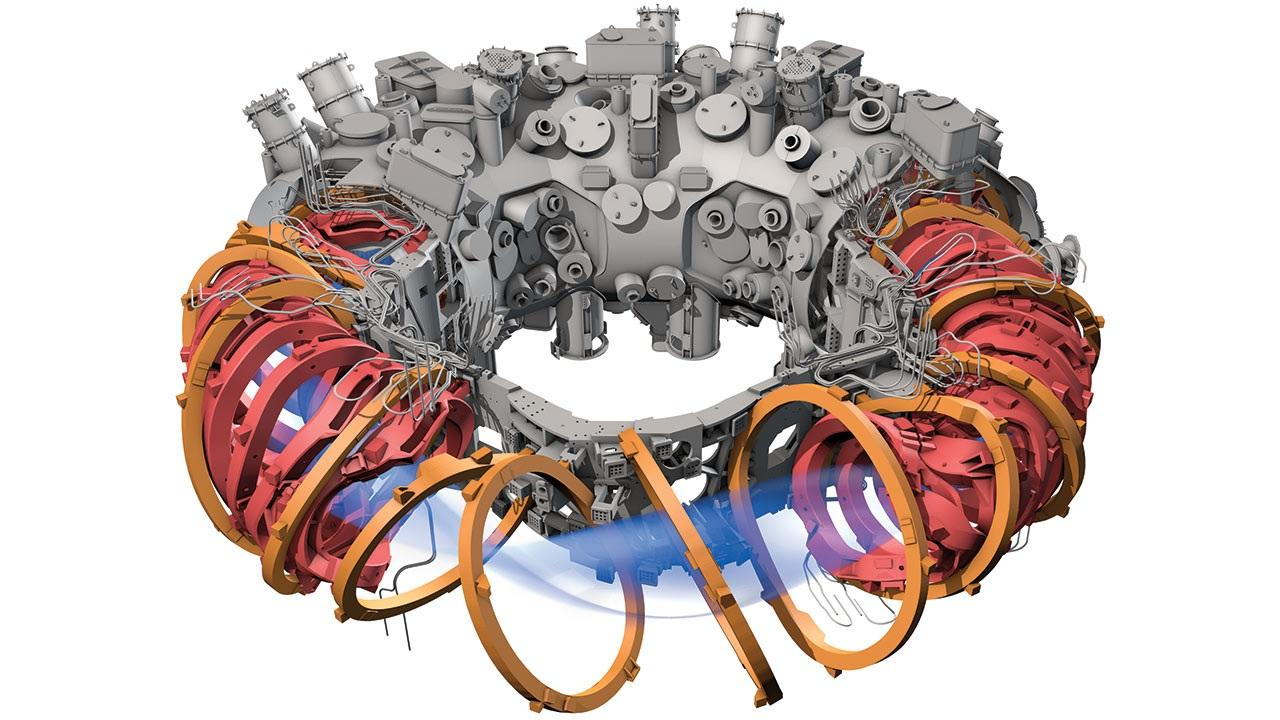
\includegraphics[width=0.9\textwidth]{graphics/stellerator.jpg}\\
  {\small Quelle: \url{http://www.sciencemag.org/news/2015/10/bizarre-reactor-might-save-nuclear-fusion} }
\end{frame}

\begin{frame}{Anwendung: Kosmologie / Astrophysik}
  \centering
  Simulation der Galaxie M74 über 13 Milliarden Jahre\\ \vspace{0.2cm}
  
\includegraphics[width=0.9\textwidth]{graphics/m74_simulation.png}\\
  {\small Quelle: \url{http://www.hpc-ch.org/first-realistic-simulation-of-the-formation-of-the-milky-way-computed-at-cscs/} }  
\end{frame}

\begin{frame}{Anwendung: Hochenergiephysik - LHC}
  \centering
  Kollision im ATLAS-Experiment\\ \vspace{0.2cm}
  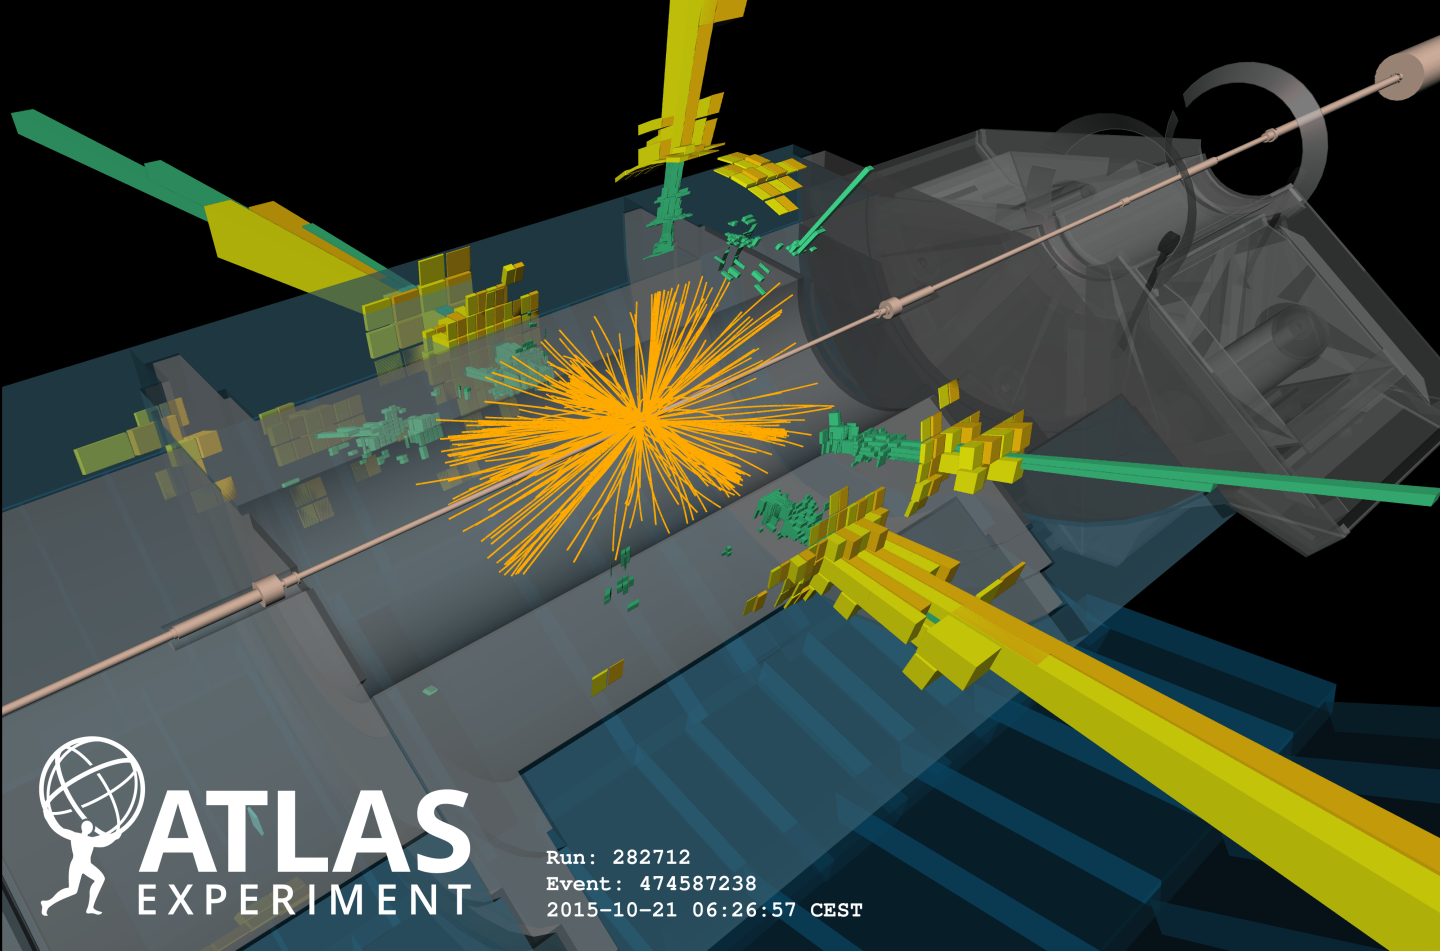
\includegraphics[width=0.9\textwidth]{graphics/atlas_event.png}\\
  {\small Quelle: \url{ https://cds.cern.ch/record/2113241 } }
\end{frame}

\begin{frame}{Anwendung: Hochenergiephysik / Gitter-QCD}
  \centering
  Simulation der Quantenchromodynamik auf Hochgeschwindigkeitsrechnern\\ \vspace{0.2cm}
  \begin{columns}
  \column{0.49\textwidth}
    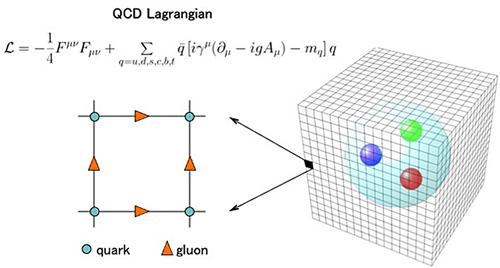
\includegraphics[width=0.8\textwidth]{graphics/LQCD2.jpg} \\
  \column{0.49\textwidth}
    
\includegraphics[width=0.8\textwidth]{graphics/juqueen.jpg} \\
  \end{columns}
  \vspace{0.3cm}
  {\small Quellen: \url{http://lpc-clermont.in2p3.fr/IMG/theorie/LQCD2.jpg} \\
                   \url{http://www.fz-juelich.de/ias/jsc/EN/Expertise/Supercomputers/JUQUEEN/JUQUEEN_node.html} }
\end{frame}

\begin{frame}{Anwendung: Biophysik / Biochemie - Molekulardynamik}
  \centering
  Simulation des NMDA Proteins und Rezeptors im menschlichen Gehirn\\ \vspace{0.2cm}
  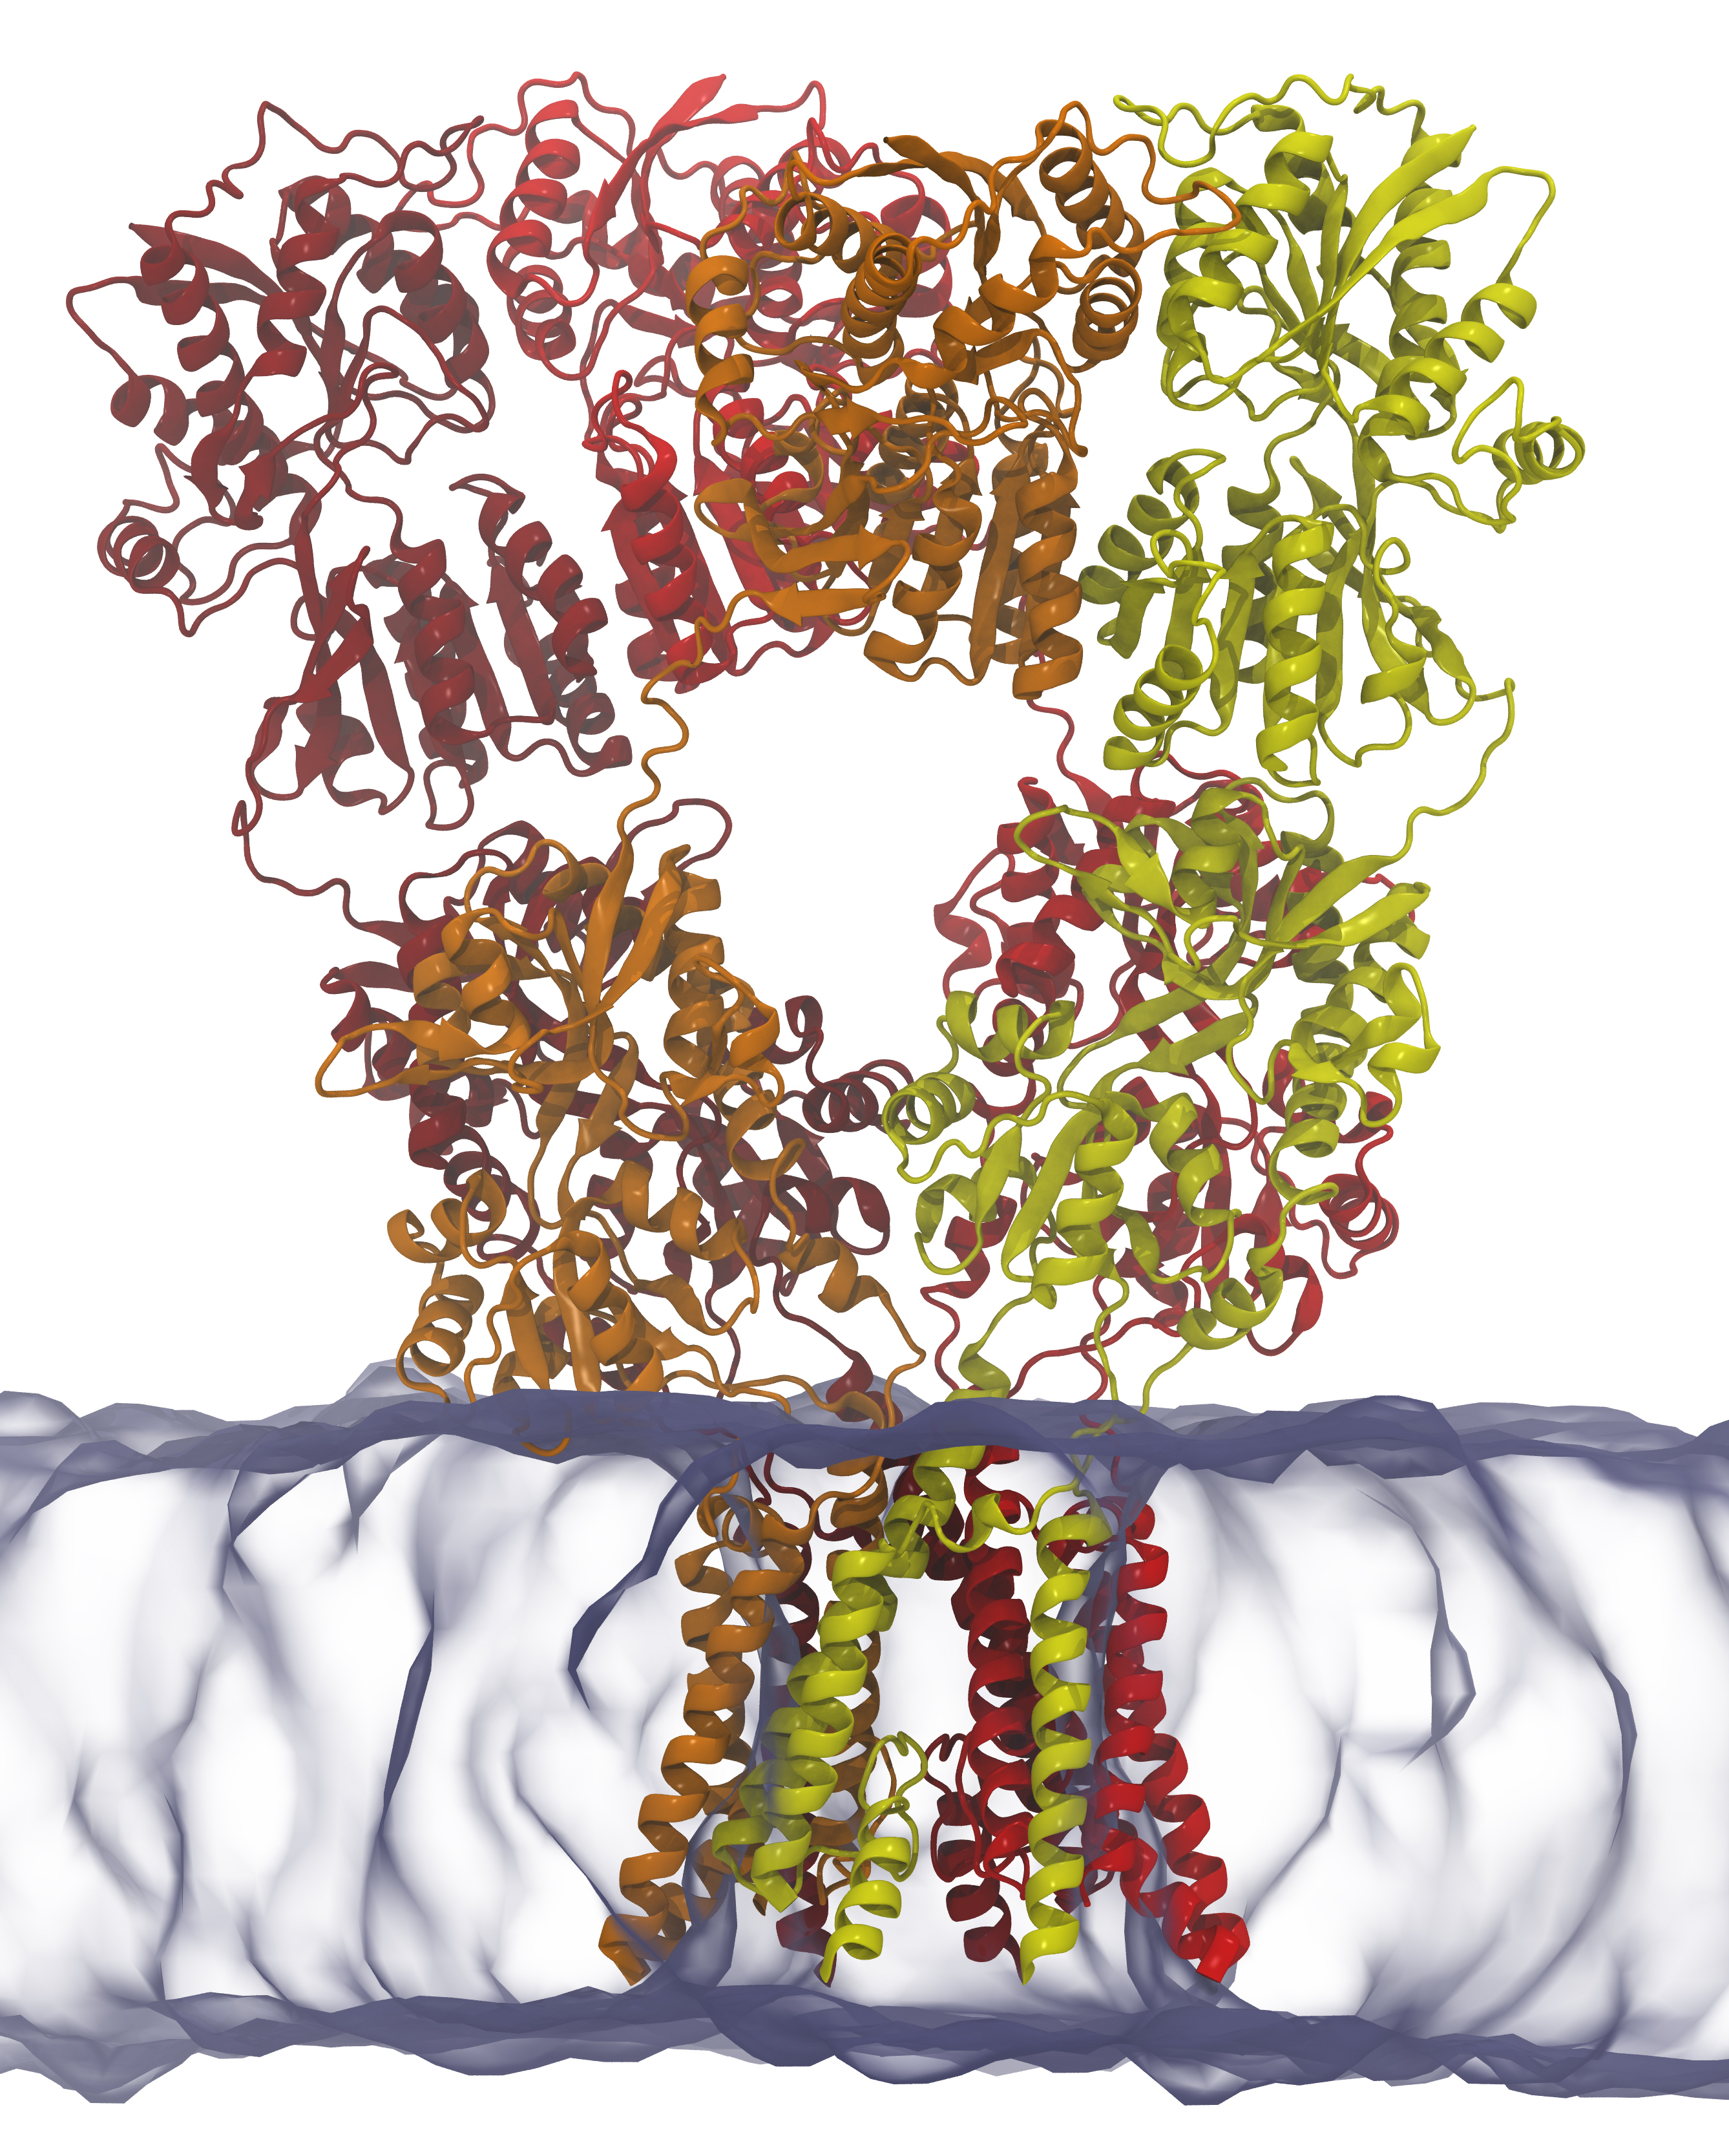
\includegraphics[width=0.4\textwidth]{graphics/glutamate.jpg}\\
  {\small Quelle: \url{http://computation.llnl.gov/glutamate-receptor-molecular-dynamics-simulation} }
\end{frame}

\begin{frame}{Die Programmiersprache C}{Vorlesung \arabic{lecturecounter}}
  \centering
  
\includegraphics[height=7cm]{graphics/The_C_Programming_Language_cover}
\end{frame}

\begin{frame}{Algorithmus: Einfügensortieren Pseudocode}{Vorlesung \arabic{lecturecounter}}
  \begin{algorithmic}
  \Procedure{insertionsort}{$U,S$}
    \State \textbf{Input:} Lists $U,S$
    \State \textbf{Output:} List $S$
    \For {$i=0$ \textbf{to} \textbf{length}(U)-$1$}
      \State $S_i \gets U_i$
      \State $j \gets i$
      \While {$j > 0$}
        \If{ $S_j < S_{j-1}$}
          \State $t \gets S_j$
          \State $S_j \gets S_{j-1}$
          \State $S_{j-1} \gets t$
          \State $j \gets j-1$
        \Else
          \State \textbf{break}
        \EndIf
      \EndWhile
    \EndFor
  \EndProcedure
\end{algorithmic}

\end{frame}

\begin{frame}[fragile]{Die Struktur eines C-Programms}{Vorlesung \arabic{lecturecounter}}
Das einfache Programm
\begin{lstlisting}
#include <stdio.h>
int main(void){
  printf("Hallo, Welt!\n");
  return 0;
}
\end{lstlisting}
können wir in einer Textdatei \verb|hallo_welt.c| abspeichern und mit dem C-Compiler in ein ausführbares Programm übersetzen
\begin{verbatim}
$ gcc -Wall -Wpedantic -std=c99 -o hallo_welt hallo_welt.c
\end{verbatim}
und es dann ausführen
\begin{verbatim}
$ ./hallo_welt
Hallo, Welt!
$ _
\end{verbatim}
\end{frame}

\begin{frame}[fragile]{Variablen deklarieren und definieren}{Vorlesung \arabic{lecturecounter}}
 Eine Variable wird in C mit:
\begin{lstlisting}
DATENTYP NAME;        // deklariert
NAME = WERT;          // definiert
DATENYP NAME = WERT;  // deklariert und definiert
\end{lstlisting}
 \begin{block}{Blöcke und Sichbarkeitsbereich (\emph{scope})}
 In C werden Programmblöcke mit $\lbrace$ und $\rbrace$ umklammert.
 Ein Block fasst mehrere Ausdrücke (\emph{statements}) zu einem Ausdruck zusammen.
 Eine Variablendeklaration gilt innerhalb eines Blocks und seiner Unterblöcke.
 \end{block}
\begin{lstlisting}
DATENTYP1 VAR1 = WERT1;         // Aeusserster Block
{
  DATENTYP2 VAR2 = WERT2;
  // hier gelten sowohl VAR1 als auch VAR2
  {
    DATENTYP3 VAR3 = WERT3;
    // hier gelten alle drei Variablen
  } // ab hier gilt VAR3 nicht mehr
} // jetzt gilt auch VAR2 nicht mehr
\end{lstlisting}
\end{frame}

\begin{frame}[fragile]{Einrückung und Kommentare}{Vorlesung \arabic{lecturecounter}}
\begin{lstlisting}
DATENTYP1 VAR1 = WERT1;         // Aeusserster Block
{
  DATENTYP2 VAR2 = WERT2;
  // hier gelten sowohl VAR1 als auch VAR2
  {
    DATENTYP3 VAR3 = WERT3;
    // hier gelten alle drei Variablen
  } // ab hier gilt VAR3 nicht mehr
} // jetzt gilt auch VAR2 nicht mehr
\end{lstlisting}
\begin{block}{}
  Ein wichtiger Aspekt, der zur Lesbarkeit eines Quelltextes beiträgt, ist eine konsistente Einrückung der Programmblöcke. Man hätte auch folgendes schreiben können.
\end{block}
\begin{lstlisting}
DATENTYP1 VAR1=WERT1;{DATENTYP2 VAR2=WERT2;{DATENTYP3 VAR3=WERT3;}}
\end{lstlisting}
\begin{block}{}
An nicht-trivialen Stellen des Programmcodes ist es zudem wichtig, dass man Kommentare einfügt, um sich und anderen zu erklären, was da geschieht. 
\end{block}
\end{frame}

\stepcounter{lecturecounter}

% \begin{frame}{Fragen zu Vorlesung 1}
%   In der letzten Vorlesung:
%   \begin{itemize}
%     \item{Rechnerarchitektur}
%     \item{Dualsystem}
%     \item{Fließkommazahlen}
%     \item{Einführung in Algorithmen und Pseudocode}
%   \end{itemize}
% 
% \end{frame}

\begin{frame}[fragile]{Bedingte Ausführung: \texttt{if / else} Statement}{Vorlesung \arabic{lecturecounter}}
\begin{block}{}
  Das \texttt{if / else} statement erlaubt es, den Programmfluss abhängig vom momentanen Zustand zu steuern.
\end{block}
Input: $x, y, z$
\begin{lstlisting}
if( x > 0 ){
  // x groesser 0
} else if ( x == 0 && y <= 1 ) {
  // x gleich 0 UND y kleiner-gleich 1
  if( (z + 3) == y ){
    // z+3 gleich y
  }
} else if ( x == 0 && y > 1 ) {
  // x gleich 0 UND y groesser 1
} else if ( x < 0 ) {
  // Falls x kleiner 0
}
if( z > 0 || (y % 2 == 0) ){
  // z groesser 0 ODER y gerade
}
\end{lstlisting}
\textbf{Unter welchen Umständen wird keine Anweisung ausgeführt?}
\end{frame}

\begin{frame}[fragile]{Schleifen: \texttt{while} \& \texttt{do-while} (1/2)}{Vorlesung \arabic{lecturecounter}}
\begin{block}{}
  Iterative Verfahren sind ein zentraler Bestandteil vieler Algorithmen.
  Schleifen wiederholen Anweisungen, bis eine gewählte Bedingung erreicht ist.
\end{block}
Die \texttt{while}- und \texttt{do-while}-Schleifen sind die einfachsten Schleifentypen in C und haben folgende Struktur:
\vspace{0.2cm}
\begin{columns}
\column{0.49\textwidth}
\begin{lstlisting}
while( LOGISCHER AUSDRUCK ){
  BEFEHLE
}  
\end{lstlisting}
\begin{enumerate}
  \item[(1)]{ \texttt{AUSDRUCK} auf Wahrheit prüfen }
  \begin{itemize}
    \item[wahr]{ \texttt{BEFEHLE} ausführen }
    \begin{itemize}
      \item[$\drsh$]{Zurück zu (1)}
    \end{itemize}
    \item[unwahr]{ Schleife beenden }
  \end{itemize}
\end{enumerate}

\column{0.49\textwidth}
\begin{lstlisting}
do {
  BEFEHLE
} while( LOGISCHER AUSDRUCK ); 
\end{lstlisting}
\begin{enumerate}
  \item[(0)]{ \texttt{BEFEHLE} ausführen }
  \item[(1)]{ \texttt{AUSDRUCK} auf Wahrheit prüfen }
  \begin{itemize}
    \item[wahr]{ zurück zu (0) }
    \item[unwahr]{ Schleife beenden }
  \end{itemize}
\end{enumerate}

\end{columns}

\end{frame}

\begin{frame}[fragile]{Schleifen: \texttt{while} \texttt{do-while} (2/2)}{Vorlesung \arabic{lecturecounter}}
\begin{block}{}
Wir wollen folgende unendliche Summe berechnen:
\begin{equation*}
  S=\sum_{n=0}^\infty x^n, \quad |x| < 1
\end{equation*}
\end{block}

\begin{lstlisting}
const double x = 0.8;         // x ist eine Konstante
double S = 0.0;               // x^0 = 1.0
double xn = 1.0;              // x^0 = 1.0
while( xn > 1.0e-12 ){        // Test auf x^n > 1,0 * 10^{-12}
  S = S + xn;
  xn = xn * x;                // x^n
}
\end{lstlisting}
\begin{lstlisting}
do {
  S += xn;
  xn *= x;
while( xn > 1.0e-12 );
\end{lstlisting}

\end{frame}

\begin{frame}[fragile]{Schleifen: \texttt{for} (1/2)}{Vorlesung \arabic{lecturecounter}}
\begin{block}{}
  In C hat eine \texttt{for}-Schleife Kontrollelemente im Schleifenkopf, ideal um mit einer Zählvariable zu arbeiten (aber auch andere Konstrukte sind möglich).
\end{block}
\begin{lstlisting}
for( INITIALISIERUNG; LOGISCHER AUSDRUCK; SCHRITT ){
  BEFEHLE
}
\end{lstlisting}
\begin{enumerate}
  \item[(0)]{\texttt{INITIALISIERUNG} wird ausgeführt}
  \begin{enumerate}
    \item[(1)]{\texttt{LOGISCHER AUSDRUCK} wird auf Wahrheit geprüft}
    \begin{enumerate}
      \item[wahr]{Weiter zu (2)}
      \item[unwahr]{Schleife beenden}
    \end{enumerate}
    \item[(2)]{\texttt{BEFEHLE} werden ausgeführt}
    \item[(3)]{\texttt{SCHRITT} wird ausgeführt}
    \item[$\Rightarrow$]{Zurück zu (1)}
  \end{enumerate}
\end{enumerate}
\end{frame}

\begin{frame}[fragile]{Schleifen: \texttt{for} (2/2)}{Vorlesung \arabic{lecturecounter}}
\begin{block}{}
Die Berechnung der Summe $\sum_{n=0}^{\infty} \, x^n$, könnte man, z.B. so implementieren:
\end{block}
\begin{lstlisting}
const double x = 0.8;
double S = 0.0;
double xn = 1.0;
for( unsigned int n = 0; n < 1000; ++n ){  // max. 1000 Iterationen
  S = S + xn;
  if( xn < 1.0e-12 ){
    break;                        // aus der Schleife ausbrechen
  }                               // selbst wenn n < 1000
  xn = xn * x;
}
\end{lstlisting}

\begin{block}{}
Oder aber auch so:
\end{block}
\begin{lstlisting}
const double x = 0.8;
double S = 0.0;
for( double xn = 1.0; xn > 1.0e-12; xn *= x){
  S += xn;
}
\end{lstlisting}
\end{frame}


\begin{frame}[fragile]{Funktionen (1/3): Definition}{Vorlesung \arabic{lecturecounter}}
\begin{block}{}
In der letzten Vorlesung hatten wir ein Programm entwickelt um eine Annäherung an die unendliche Summe
\begin{equation*}
  S=\sum_{n=0}^\infty x^n, \quad |x| < 1
\end{equation*}
zu bestimmen. Wir können mit einer Funktion die Berechnung verallgemeinern.
\end{block}
\begin{lstlisting}
double sum_xn( const double x, const unsigned int nmax, 
               const double tolerance ){
  double S = 0.0;
  double xn = 1.0;
  for( unsigned int n = 0; n < nmax; ++n ){  
    S += xn;
    if( xn < tolerance ){
      break;                        
    }                               
  xn *= x; 
  }
  return S;
}
\end{lstlisting}
\end{frame}

\begin{frame}[fragile]{Funktionen (2/3): Funktionskopf und Signatur}{Vorlesung \arabic{lecturecounter}}
\begin{block}{}
  Eine Funktion wird dem Compiler bekannt gemacht, indem ihr Name und die Datentypen ihrer Argumente festelegt werden. $\Rightarrow$ \emph{Funktionsdeklaration}
\end{block}

\begin{lstlisting}
RUECKGABETYP FUNKTIONSNAME( ARGUMENT1_TYP ARG1, ARGUMENT2_TYP ARG2,
                            ARGUMENT3_TYP ARG3 );
\end{lstlisting}
\begin{block}{Signatur}
  {\footnotesize \verb| (FUNKTIONSNAME) ( ARGUMENT1_TYP, ARGUMENT2_TYP, ARGUMENT3_TYP ) | }
\end{block}

\begin{block}{}
  Wichtig: Bei der Unterscheidung zweier Funktionen gleichen Namens, wird der Typ des Rückgabewerts \emph{nicht} berücksichtigt!
\end{block}
\begin{lstlisting}
double teilen( double zaehler, double nenner ){ [...] }
float  teilen( double zaehler, double nenner ){ [...] } // Fehler!
float  teilen( float  zaehler, float  nenner ){ [...] } // OK
\end{lstlisting}
\end{frame}

% \begin{frame}[fragile]{Funktionen (3/3): Funktionsaufruf und Rekursion}{Vorlesung \arabic{lecturecounter}}
% \end{frame}

\end{document}
